\section{Aufgabe 14: Hauptkomponentenanalyse}
\subsection{a)}
(Siehe Python-Datei) In Abbildung \ref{abb:1} ist die gegebene Verteilung
für die 1. und die 4. Dimension gegeneinander aufgetragen.
\begin{figure}
  \centering
  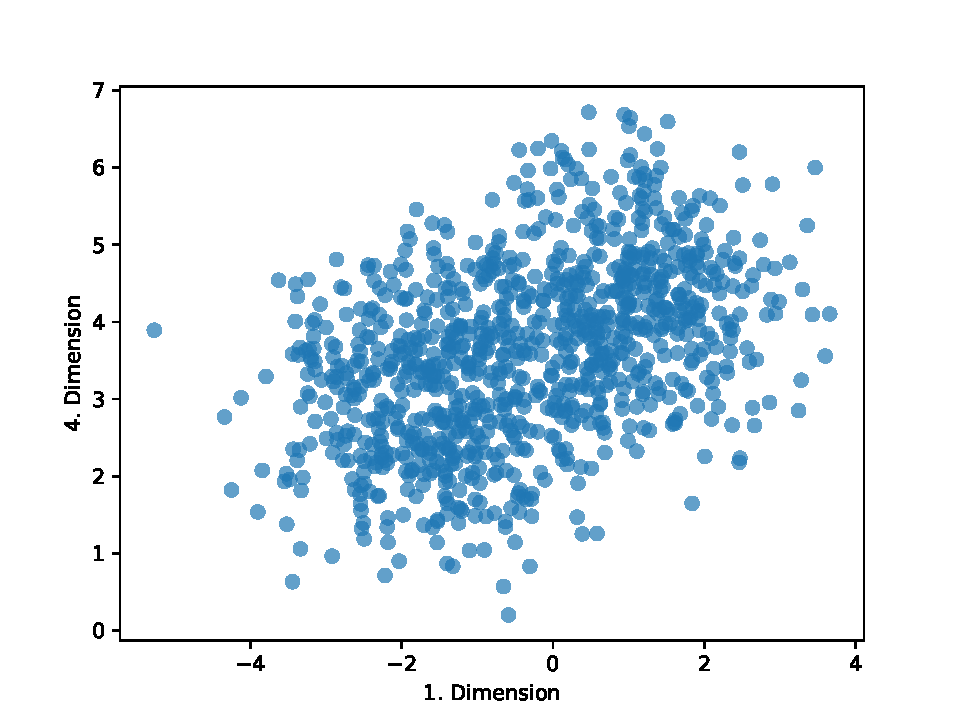
\includegraphics[scale=0.7]{Aufgabe14/Scatterplot.pdf}
  \caption{Scatterplot.}
  \label{abb:1}
\end{figure}


\subsection{b)}
Die Hauptkomponentenanalyse ist dazu da, um eine n-dimensionale Verteilung
auf eine p-dimensionale Verteilung zu reduzieren (n>p) oder auch eine mehrdimensionale
Verteilung zu dekorrelieren, indem die Achsen transformiert werden. Hierbei sollen
möglichst wenige Informationen verloren gehen, wobei man mehrere korrelierende
Komponenten zu einer "Hauptkomponente" zusammenfasst.
Reihenfolge der Hauptkomponentenanalyse:
\begin{itemize}
  \item Zentrieren der Daten auf den Nullpunkt
  \item Berechnung der Kovarianzmatrix
  \item Berechnung der der Eigenwerte und der Eigenverktoren der Kovarianzmatrix
  \item Wähle die k größten Eigenwerte und zugehörigen Eigenvektoren aus
  \item Bilde eine d x k Matrix W mit den k Eigenvektoren als Spalten
  \item Wende W auf jede Zeile aus $x$ aus $X$ an $x' = W^T \cdot x^T$
\end{itemize}

\subsection{c)}
(Siehe Python-Datei) Die Kovarianzmatrix:

\begin{align*}
  \symup{Cov} = \begin{pmatrix}
                 2.63 &  0.80 &  2.12 & -4.38  \\
                 0.80 &  1.34 &  1.10 & -2.19 \\
                 2.12 &  1.10 &  3.70 & -5.66 \\
                -4.38 & -2.19 & -5.66 & 12.75 \\
  \end{pmatrix}
\end{align*}

Die Eigenwerte der Kovarianzmatrix:
\begin{align*}
  \lambda_1 = 17.52 \\
  \lambda_2 = 0.90 \\
  \lambda_3 = 1.00 \\
  \lambda_4 = 17.52 \\
\end{align*}

Die Hauptkomponente mit dem größten Eigenwert (hier $\lambda_1$) ist am
signifikantesten, falls eine Reduktion der Dimensionen vorgenommen werden soll.
Die anderen Dimensionen haben nur einen Eigenwert von etwas unter 1 und sind somit
viel kleiner als der der ersten Dimension.

\subsection{d)}
in Abbildung \ref{abb:2} ist der Scatterplot abgebildet.

\begin{figure}
  \centering
  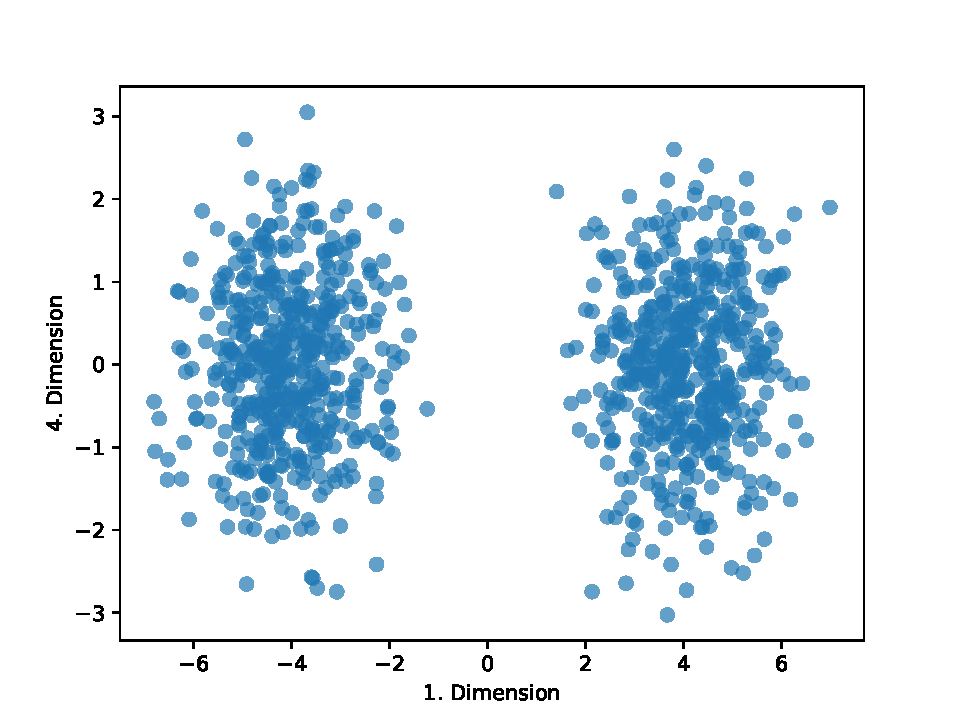
\includegraphics[scale=0.7]{Aufgabe14/Scatterplot_pca.pdf}
  \caption{Scatterplot}
  \label{abb:2}
\end{figure}

In Abbildung \ref{abb:3} und \ref{abb:4} sind die Histogramme der Dimensionen
vor und nach der PCA dargestellt.

\begin{figure}
  \centering
  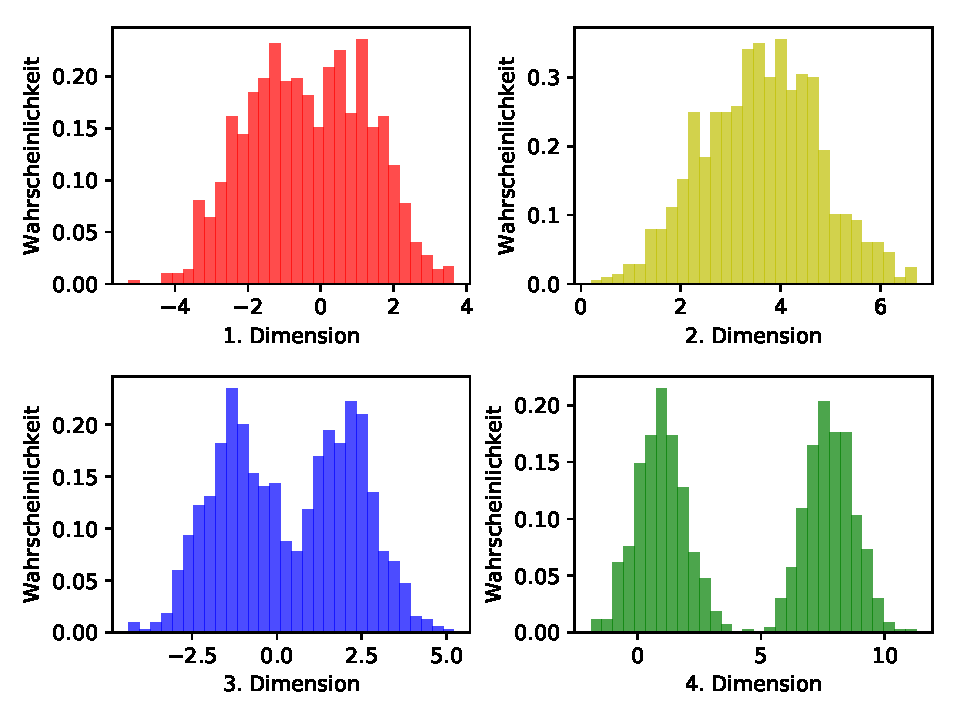
\includegraphics[scale=0.7]{Aufgabe14/Histogramm_vorher.pdf}
  \caption{Histogramm vorher}
  \label{abb:3}
\end{figure}
\begin{figure}
  \centering
  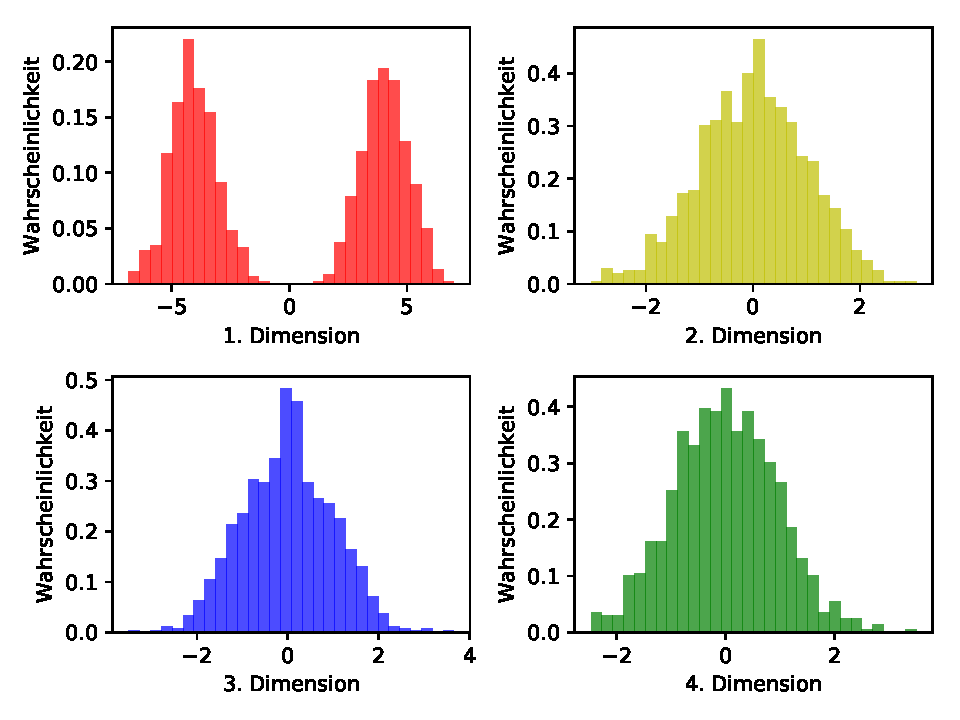
\includegraphics[scale=0.7]{Aufgabe14/Histogramm.pdf}
  \caption{Histogramm nachher}
  \label{abb:4}
\end{figure}
